% =====
% Conteúdo dos artefatos
% =====

% -----
% Ficha catalográfica (Obrigatório)
% -----

% Para a versão final do trabalho, sua instituição pode lhe fornecer um PDF com a versão definitiva da ficha catalográfica.

% Se for este o caso, salve o PDF no diretório "documentos" do seu projeto, então utilize a segunda versão do comando abaixo.

% Substitua "documentos/black-square.pdf" pelo caminho do PDF que você salvou no seu projeto.

\insereFichaCatalografica%
% \insereFichaCatalografica[%
%     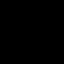
\includepdf{documentos/black-square.pdf}
% ]

% -----

% -----
% Errata
% -----

\insereErrata{%
    \lipsum[1]

    \lipsum[8]
}

% -----

% -----
% Folha de aprovação (Obrigatório)
% -----

\insereFolhaDeAprovacao%

% Caso haja muitos membros na banca, e o espaço para as assinaturas na página fique pequeno, habilite a versão do comando abaixo.
% Isso fará com que a lista de membros da banca seja impressa em duas colunas.

% \insereFolhaDeAprovacaoEmDuasColunas%

% Para a versão final do trabalho, sua instituição pode lhe fornecer um PDF com a versão definitiva da folha de aprovação.

% Se for este o caso, salve o PDF no diretório "documentos" do seu projeto, então utilize a segunda versão do comando abaixo.

% Substitua "documentos/black-square.pdf" pelo caminho do PDF que você salvou no seu projeto.

% \insereFolhaDeAprovacao[%
%     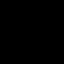
\includepdf{documentos/black-square.pdf}
% ]

% -----

% -----
% Dedicatória (Opcional)
% -----

\insereDedicatoria{%
    Este trabalho é dedicado às crianças adultas que, quando pequenas, sonharam em se tornar cientistas.
}

% -----

% -----
% Agradecimentos (Opcional)
% -----

\insereAgradecimentos{%
    Agradecemos ao projeto \abnTeX\footnote{%
        Acesso em:~\url{http://www.abntex.net.br/}.%
    }, que disponibiliza o modelo \LaTeX\ que foi customizado para a elaboração de trabalhos acadêmicos conforme as normas da ABNT.

    Agradecemos também ao professor Dr.\ Jairo Souza, que desenvolveu o modelo \LaTeX\ para o \gls{dcc} da \gls{ufjf}, o qual baseou partes deste modelo.
}

% -----

% -----
% Epígrafe (Opcional)
% -----

% A epígrafe é necessariamente uma citação de outro autor. A obra referenciada deve estar na bibliografia.

% Caso a epígrafe tenha mais de 3 linhas, ative o ambiente "citacao" abaixo, para formatá-la conforme as normas da ABNT.

\insereEpigrafe{%
    % \begin{citacao}
    ``Mathematical reasoning may be regarded rather schematically as the exercise of a combination of two facilities, which we may call intuition and ingenuity''~\cite{turing:1939}.
    % \end{citacao}
}

% -----

% -----
% Resumo (Obrigatório)
% -----

% --- Língua vernácula ---

% Palavras chave. Parâmetros: palavra-chave um; palavra-chave dois; palavra-chave três; palavra-chave quatro (opcional); palavra-chave cinco (opcional). Deixe em branco os campos opcionais que não deseja preencher.
\DefinePalavrasChave{palavra um}{palavra dois}{palavra três}{palavra quatro}{}

\insereResumo{%
    \lipsum[1-3]

    \lipsum[11-13]
}

% --- Língua estrangeira ---

% Parâmetros: língua (english, french, spanish, italian, german, dutch); palavras-chave; conteúdo.

\insereResumoEmLinguaEstrangeira%
{english}
{\formataPalavrasChave{word one}{word two}{word three}{word four}{}}
{%
    \lipsum[4-6]

    \lipsum[14-16]
}

\insereResumoEmLinguaEstrangeira%
{french}
{\formataPalavrasChave{word one}{word two}{word three}{word four}{}}
{%
    \lipsum[30-32]

    \lipsum[34-36]
}

% -----

% -----
% Glossário (Opcional)
% -----

% Comente para remover o glossário.
\insereGlossario{}

% -----

% =====
